\section{TP1 : Transmission "back-to-back" - Mise en place de l'infrastructure}
\sectionmark{TP1 : Transmission "back-to-back" - Mise en place de l'infrastructure}

\subsection{Introduction étape 1}


Cette étape est la première de ce projet, nous ayant permis de prendre en main l'architecture logicielle et des livrables à prévoir.

La transmission est, dans ce premier livrable, parfaite. Le calcul du T-E-B est donc pour l'instant inutile (malgré qu'il ait été implémenté), puisque toujours égal à 0 dans cette étape quelles que soit les conditions.

\subsection{Mise en oeuvre}


\begin{figure}[H]
    \centering
    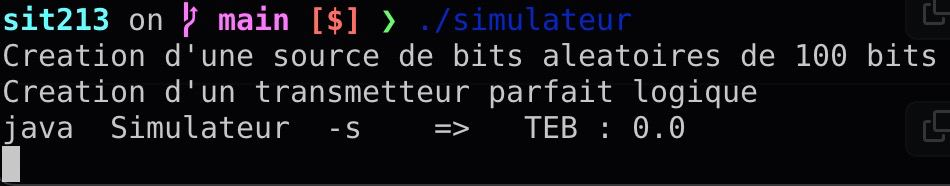
\includegraphics[width=0.5\textwidth]{img/etape1_teb1.jpg}
    \caption{Taux d'erreur binaire pour une source aléatoire de 100 bits}
    \label{fig:teb1}
\end{figure}
\begin{figure}[H]
    \centering
    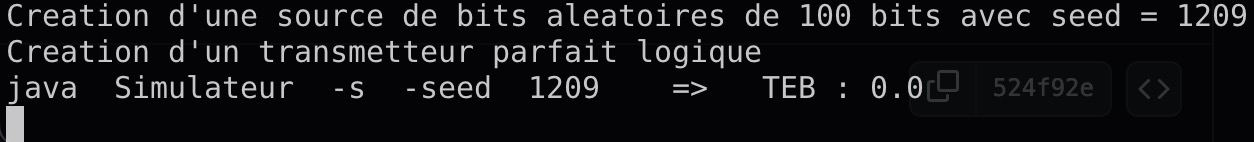
\includegraphics[width=0.5\textwidth]{img/etape1_teb3.jpg}
    \caption{Taux d'erreur binaire pour une source aléatoire avec seed}
    \label{fig:teb2}
\end{figure}
\begin{figure}[H]
    \centering
    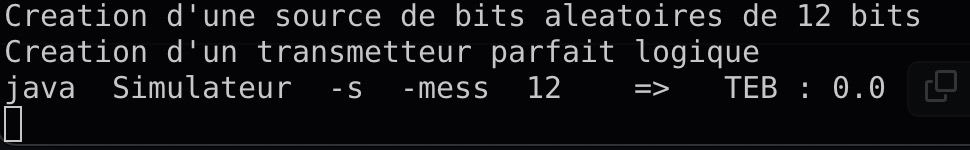
\includegraphics[width=0.5\textwidth]{img/etape1_teb2.jpg}
    \caption{Taux d'erreur binaire pour une source fixé par l'utilisateur}
    \label{fig:teb3}
\end{figure}
\begin{figure}[H]
    \centering
    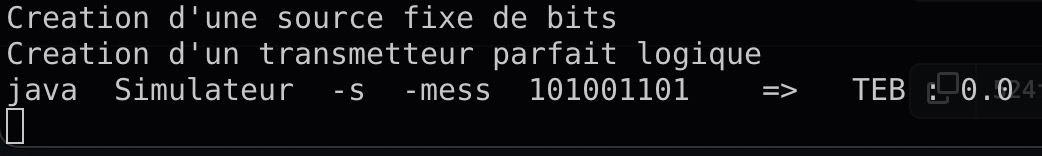
\includegraphics[width=0.5\textwidth]{img/etape1_teb4.jpg}
    \caption{Taux d'erreur binaire pour une source fixé par l'utilisateur (en binaire)}
    \label{fig:teb4}
\end{figure}


Ainsi on observe dans les 4 cas :
\begin{itemize}
    \item Message liés à la génération de 100 symboles aléatoires à l'exécution ;
    \item Message liés à la génération de 100 symboles aléatoires à partir d'une seed fixée par l'utilisateur (\texttt{-seed [chaîne de caractères]}) ;
    \item Message fixés par l'utilisateur (\texttt{-mess [chaîne de caractères]}) ;
\end{itemize}

que le résultat de la transmission dans notre simulation est l'exact réplique de la source.

\begin{figure}[H]
    \centering
    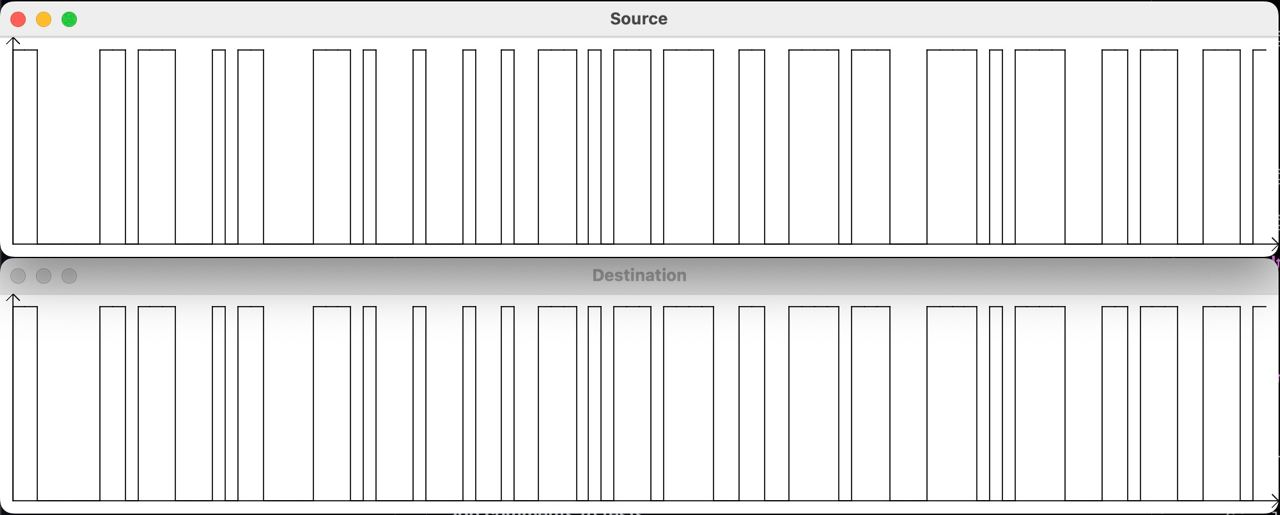
\includegraphics[width=\textwidth]{img/etape1_source_et_dest.jpg}
    \caption{Résultat d'une simulation entre source et destination}
    \label{fig:simulation1}
\end{figure}

Nos sondes ont été, en effet, placés en sortie de la source, ainsi qu'en sortie du transmetteur parfait (juste avant la destination finale).

Les résultats de la simulation correspondent bien aux attentes de l'énoncé et aux prévisions que l'on pouvait avoir avant la réalisation de celle-ci.

\subsection{Conclusion étape 1}

Pour cette première itération, les résultats sont donc conformes aux attendus, et l'objectif de compréhension de l'architecture logicielle ainsi que des attendus du livrable ont été respectés.

L'intégration des tests JUnit dès cette première étape nous permettra par la suite d'aisément travailler en Développement Dirigé par les Tests et garantir, ainsi, la qualité de notre code et sa conformité, ainsi que d'éviter des régressions sur les codes déjà livrés.

